This layer processes the data scanned from the presentation layer and stores the data in local variables, i.e. name 
of the beverage and expiry date. This data is added to the current user's beverage database and send the updated data
back to the presentation layer for further input.

\subsection{Subsystem 1}
This section should be a general description of a particular subsystem for the given layer. For most subsystems, 
an extract of the architectural block diagram with data flows is useful. This should consist of the subsystem 
being described and those subsystems with which it communicates.

\begin{figure}[h!]
	\centering
 	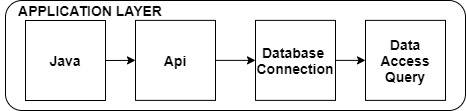
\includegraphics[width=0.60\textwidth]{images/App.jpg}
 \caption{Example subsystem description diagram}
\end{figure}

\subsubsection{Assumptions}
\begin{itemize}
    \item The drink is in the database of drinks
    \item The data inputted is correct.
\end{itemize}

\subsubsection{Responsibilities}
Each of the responsibilities/features/functions/services of the subsystem as identified in the architectural 
summary must be expanded to more detailed responsibilities. These responsibilities form the basis for the 
identification of the finer-grained responsibilities of the layer's internal subsystems. Clearly describe what 
each subsystem does.

\subsubsection{Subsystem Interfaces}
Each of the inputs and outputs for the subsystem are defined here. Create a table with an entry for each labelled 
interface that connects to this subsystem. For each entry, describe any incoming and outgoing data elements will 
pass through this interface.

\begin {table}[H]
\caption {Subsystem interfaces} 
\begin{center}
    \begin{tabular}{ | p{1cm} | p{6cm} | p{3cm} | p{3cm} |}
    \hline
    ID & Description & Inputs & Outputs \\ \hline
    \#xx & Description of the interface/bus & \pbox{3cm}{input 1 \\ input 2} & \pbox{3cm}{output 1}  \\ \hline
    \#xx & Description of the interface/bus & \pbox{3cm}{N/A} & \pbox{3cm}{output 1}  \\ \hline
    \end{tabular}
\end{center}
\end{table}

\subsection{Subsystem 2}
Repeat for each subsystem

\subsection{Subsystem 3}
Repeat for each subsystem

